\chapter{Overview of Data Resources}

Data stands as the cornerstone of both precision medicine and machine learning.
Its availability is crucial; without it, research in these
fields would be almost impossible. 
The emergence of high-throughput analyses and \acp{EHR} has 
led to a Cambrian explosion of the volume of data being generated,
which has the potential of revolutionizing the 
entire landscape of biomedical research. 
However, the sensitive nature of this data means
that access is frequently a major challenge, 
often serving as a major bottleneck in
many research endeavors.

In the context of the studies conducted for this thesis, I have been in the
privileged position of working within a research group where permissions, 
data access, and the necessary infrastructure were already well-established.
In terms of infrastructure, a key aspect of our data handling involved the use 
of a secure high-performance computing environment. 
This not only ensured the efficient processing of large datasets and 
training of large neural networks, 
but also maintained the highest standards of data security and
confidentiality, which are paramount in dealing with sensitive health records.
These aspects have been instrumental in enabling and driving 
the research and analyses presented in this thesis.

Focusing on the data itself,
this chapter aims to provide a comprehensive overview of the various data
sources utilized in the studies comprising this thesis. It details the
databases and registries that were accessed and analyzed,
highlighting how each contributed to the research. 

\begin{figure*}
\begin{tikzpicture}[
    x=\linewidth,
    tbox/.style={minimum height=5mm, thick, yshift=1em, inner sep=0pt},
    ttex/.style={color=black, font=\sffamily},
]
    \foreach \year 
        [evaluate=\year as \x using (\year-1965)/(2025-1965)] 
            in {1965, 1966, ..., 2025} \node [anchor=center] (\year) at (\x, 0) {};

    \draw [->] (1965) -- (2025) node[midway, below] (timeline) {};

    % labels
    \node [below] at (1968) {1968};
    \node [below] at (1977) {1977};
    \node [below] at (1994) {1994};
    \node [below] at (2023) {2023};
    \node [below] at (2000) {2000};
    \node [below] at (2006) {2006};
    \node [below] at (2016) {2016};

    \node [tbox, fit={(1968 |- 0,1ex)   (2023 |- 0,1ex)},   fill=color2] (1) {};
    \node [tbox, fit={(1970 |- 1.north) (2023 |- 1.north)}, fill=color3] (2) {};
    \node [tbox, fit={(1977 |- 2.north) (1994.west |- 2.north)}, fill=color4] (3) {};
    \node [tbox, fit={(1994.east |- 2.north) (2023 |- 2.north)}, fill=color4] (4) {};
    \node [tbox, fit={(2000 |- 4.north) (2023 |- 4.north)}, fill=color5] (5) {};
    \node [tbox, fit={(2006 |- 5.north) (2016 |- 5.north)}, 
            draw=black, fill=color6] (6) {};

    % \draw [dashed] (2006) -- (6.north west);
    % \draw [dashed] (2016) -- (6.north east);

    \node [ttex] at (1.center) {CPR};
    \node [ttex] at (2.center) {DAR};
    \node [ttex] at (3.center) {DNPR (ICD-8)};
    \node [ttex] at (4.center) {DNPR (ICD-10)};
    \node [ttex] at (5.center) {EDHR};
    \node [ttex] at (6.center) {BigTempHealth};

\end{tikzpicture}
    \setfloatalignment{b}
    \caption[Overview of Data]{%
        Overview of the different data resources used in 
        the research projects presented in this thesis.
        This schematic shows the timeline of the different datasets.
        \vspace{2em}
    }
    \label{fig:data-overview}
\end{figure*}

\section{The Danish Civil Registration System}

\Ac{CPR} is the central administrative register in Denmark,
and stores personal information on the entire Danish population,
including birth date, sex, addresses, vital status, 
and, importantly, a unique personal identification number, 
known as \enquote{\ac{CPR}-nummer} or \enquote{personnummer}.
~\autocite{schmidtDanish2014}

The \ac{CPR} number is assigned at birth or upon obtaining Danish citizenship, 
and have been in use since 1968.
As of January 2, 2014, 
\num{9484792} \ac{CPR} numbers were assigned.
~\autocite{schmidtDanish2014}
Of these \num{5685912} were \enquote{active},
and \num{3798880} were \enquote{non-active},
the latter primarily attributed to death and emigration.
~\autocite{schmidtDanish2014}

In Denmark, the \ac{CPR} number is as essential as a bicycle, 
required for opening a bank account, 
borrowing a library book, 
getting treated for appendicitis, and everything in between.
This widespread use, 
combined with the country's long-standing tradition
of organising and keeping record of detailed data in 
administrative databases and registries,
have enabled the construction of a large network
of interlinkable epidemiological resources.
~\autocite{schmidtDanish2019}
In this light, the whole nation can be utilized as a research cohort,
as outlined by \textcite{frankEpidemiology2000} in a letter
to \textit{Science}.

Linkage between the different data sources and registries presented 
throughout this thesis relied on the use of the \ac{CPR} number,
specifically an encrypted form of it, ensuring that no actual \ac{CPR}
numbers were being handled.

\section{The Danish National Patient Register}

Of the Danish registries, \ac{LPR} is arguably one of the most important.
\ac{LPR}, or \enquote{Landspatientregisteret}, 
is a comprehensive clinical register that has
been instrumental for clinical research and administration in Denmark,
and serves multiple critical functions.
~\autocite{schmidtDanish2015}
Primarily, it underpins the Danish Health and Medicines Authority's hospital
statistics and is a main foundation for health economic calculations.
Additionally, the \ac{LPR} is instrumental in monitoring the
prevalence of various diseases and treatments. 
Furthermore, the registry plays a key role in
facilitating quality assurance of Danish healthcare services and provides
hospital physicians access to patients' hospitalization histories, enhancing
patient care and treatment efficacy.
~\autocite{schmidtDanish2015}
The register is updated monthly based on reports from the hospitals,
and has been collecting data continuously since 1977.
~\autocite{schmidtDanish2015}

\subsection{Content and Structure}

The \ac{LPR} encompasses a wide array of data on each individual, 
such as personal information, admission and discharge details, diagnoses, 
examinations, treatments including surgeries, information on accidents, 
and additional details concerning births. 
~\autocite{schmidtDanish2015}
The information in the register is organised in a
structured format with different data types being stored 
in distinct tables that can be linked following a 
specified relational data model.
~\autocite{lpr2dok}

This data model, referred to as \acsfont{LPR2},  
have remained largely unchanged since the release of the registry in 1977.
However, in early 2019, it underwent a significant overhaul to a 
new and refined data model, \acsfont{LPR3}.
~\autocite{nielsenLPR32018}
The \acsfont{LPR3} model addresses certain limitations of its predecessor, 
notably enabling the creation of more fine-grained patient care timelines. 
While the specifics of these improvements are beyond the scope of this thesis, 
it is important to note that the \acsfont{LPR3} model is not entirely 
backwards compatible with the \acsfont{LPR2} data model. 
Nevertheless, depending on the specific use case, 
it remains possible to create data extracts that are compatible
to one another.

\subsection{Classification of Diseases}

The highly structured data within the \ac{LPR} 
is coded using the national \acs{SKS} classification scheme (\enquote{\acl{SKS}}), 
a collection of Danish, international, and Nordic classification standards
maintained by the Danish Health Data Authority.
~\autocite{schmidtDanish2015}
These standards includes
the \acfi{NOMESCO} system for surgical procedures,
the \acfi{ATC} system for medication,
and the \acfi{ICD} system for diagnoses. 
~\autocite{schmidtDanish2015}

Focusing on diagnosis codes, 
the \ac{LPR} is currently using the \ac{ICD-10},
and have been doing so since the start of 1994
where it replaced the \acsu{ICD-8}.
~\autocite{schmidtDanish2015}
This transition can complicate longitudinal studies of disease occurence, 
but prior efforts by the Brunak group have succesfully
created a mapping between \ac{ICD-8} and \ac{ICD-10}
that can be used to mitigate such challenges.
~\autocite{pedersenUnidirectional2023}
However, since the two systems are not directly compatible, 
this mapping only offers a partial solution 
and might not be universally applicable.

The \ac{ICD-10} coding system follows a hierarchical structure 
with every code beginning with a letter followed by two or more digits.
Each code falls in one of 21 high-level categorisation of diagnoses 
that e.g.  includes chapters
(ii)~\emph{Neoplasms};
(iv)~\emph{Endocrine, Nutritional, and Metabolic Diseases};
and (ix)~\emph{Diseases of the Circulatory System}.

Using the latter as an example, 
\cref{fig:icd10-hierarchy} shows the hierarchical structure of the
\ac{ICD-10}.
This hierarchical structure can be utilized in feature engineering for
machine learning applications, offering features of varying specificity. 
Following the example in \cref{fig:icd10-hierarchy},
a relatively specific \enquote{level-4} code, such as e.g. 
\emph{acute transmural myocardial infaction of the inferior wall}
(\acsfont{I21.1}), can also be represented as a \enquote{level-3} code,
a \enquote{block} code, or a \enquote{chapter} by stepping back
through the hierarchy.
This versatility aids in balancing between statistical power
and specificity of the included code.

% figure: icd10-hierarchy→
\begin{figure}
\begin{tikzpicture}[
    every node/.append style = {
        draw, anchor = west, 
        minimum width=10mm, 
        minimum height=4mm,
        font=\tlfstyle\scriptsize,
        rounded corners=1pt,
        fill=color2!5
    },
    sel/.style = {fill=color2!20, draw=black, thick},
    txt/.style = {
        fill=none, draw=none, font=\footnotesize\itshape, 
        text width=3.7cm, text height=5mm
    },
    grow via three points={
        one child    at (1.0, -0.5) and 
        two children at (1.0, -0.5) 
                    and (1.0, -1.0)
    },
    edge from parent path={
        (\tikzparentnode.east) 
        -| ([xshift=-4.2]\tikzchildnode.west)
        |- (\tikzchildnode.west)
    }]
    \node[sel] {chap. ix}
        child {node {I00-I02}}
        child {node {I05-I09}}
        child {node {I10-I15}}
        child {node[sel] {I20-I25}
            child {node (i20) {I20}}
            child {node [sel] (i21) {I21}
                child {node (1) {I21.0}}
                child {node (2) {I21.1}}
                child {node (3) {I21.3}}
                child {node (4) {I21.4}}
                child {node (5) {I21.9}}
            }
            child {node {I22}}
            child {node {I24}}
            child {node {I25}}
        }
        child {node {I26-I28}}
        child {node {I30-I52}}
        child {node {I60-I69}}
        child {node {I70-I79}}
        child {node {I80-I89}}
        child {node {I95-I99}}
    ;

    \node [txt] (t1) at (6.3cm, -1.5cm) 
        {acute transmural myocardial infarction of anterior wall};
    \node [txt, below=3mm of t1.center] (t2) 
        {acute transmural myocardial infarction of inferior wall};
    \node [txt, below=3mm of t2.center] (t3) 
        {acute transmural myocardial infarction not otherwise specified};
    \node [txt, below=3mm of t3.center] (t4) 
        {acute myocardial infarction with non-ST elevation};
    \node [txt, below=3mm of t4.center] (t5) 
        {acute myocardial infarction not otherwise specified};

    \draw (1.east) .. controls +(2ex,0) and +(-3ex,0) .. (t1.west);
    \draw (2.east) .. controls +(2ex,0) and +(-3ex,0) .. (t2.west);
    \draw (3.east) .. controls +(2ex,0) and +(-3ex,0) .. (t3.west);
    \draw (4.east) .. controls +(2ex,0) and +(-3ex,0) .. (t4.west);
    \draw (5.east) .. controls +(2ex,0) and +(-2ex,0) .. (t5.west);
    
\end{tikzpicture}
\caption[The ICD-10 Hierarchy]{%
    Schematic illustrating the hierarchical structure of the \ac{ICD-10} coding
    system. 
    Using chapter ix---which covers diseases of the circulatory system
    (codes I00-I99) and comprises ten different \enquote{blocks}---as an example, 
    the diagram shows how these blocks are segmented into 
    \enquote{level 3} codes, such as I20 to I25, 
    corresponding to ischemic heart disease. 
    It provides an expanded view of the I21 category, 
    containing specific subtypes, \enquote{level 4} codes, 
    of acute myocardial infarctions 
    from I21.0 for the anterior wall 
    to I21.9 for unspecified instances. 
    Deeper levels of the hierarchy also exists,
    but is not included in this diagram.
}
\label{fig:icd10-hierarchy}
\end{figure}
% ←

\subsection{Role in this Thesis}

The \ac{LPR} has been an key data resource in all three studies of this thesis. 
Diagnosis codes and their associated admissions timestamps were used to 
features for clustering analysis in \studyi{} 
and for machine learning models in \studyii{} and \studyiii{}.
Additionally, procedure, treatment, and examination codes played a vital role 
in defining cohorts in all studies, 
served as features in \studyii{} and \studyiii{},
and were crucial for defining outcomes in \studyi{} and \studyiii{}.

\section{The Causes of Death Register}

When someone in Denmark dies, 
it has since 1871 been mandatory by law that a physician
performs a post-mortem examination and fills in a death certificate.
~\autocite{helweg-larsenDanish2011}
Starting in 1970, these certificates have been stored electronically 
in \ac{DAR} (\enquote{dødsårsagsregisteret}),
which is the main source of data for 
Danish mortality statistics,
analyses of medical treatment,
and to define outcomes in various research projects.
~\autocite{helweg-larsenDanish2011}
The registry includes data such as 
the date of death, the primary and contributing causes
of death, as well as demographic information about the deceased.
Since 2002, the underlying cause of death have been coded using \ac{ACME},
an international standard for automated selection of such.
~\autocite{helweg-larsenDanish2011}
In \studyi{} and \studyiii{} of this thesis, 
the \ac{DAR} were used to define cause-specific mortality.


\section{The Eastern Denmark Heart Registry}

\begin{marginfigure}
    \centering
	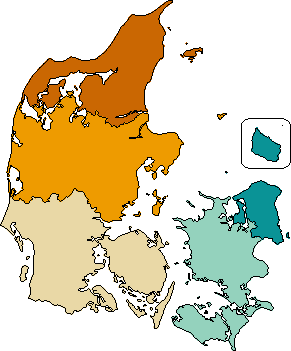
\includegraphics{graphics/regions}
    \caption[Regions of Denmark]{%
        The five administrative regions of Denmark,
        each in charge of the regional hospitals,
        are: (\,\cbox{color2}{\phantom{a}}\,) {the Capital Region of Denmark},
        (\,\cbox{color3}{\phantom{a}}\,) {Region Zealand},
        (\,\cbox{color4}{\phantom{a}}\,) {Region of Southern Denmark},
        (\,\cbox{color5}{\phantom{a}}\,) {Central Denmark Region}, and
        (\,\cbox{color6}{\phantom{a}}\,) {Northern Denmark Region}
        \vspace{1em}
    }
    \label{fig:regions}
\end{marginfigure}

The \ac{EDHR}, or \enquote{Web-PATS}, is a clinical database collecting
information on all \acp{CAG} and \acp{PCI} performed in the Capital
Region of Denmark and Region Zealand (see \cref{fig:regions}).
It collects a wide array of prognostic factors, 
demographics, administrative details, 
and procedure-related information and findings
that are used for both research and clinical quality assessment.
~\autocite{ozcanDanish2016}

In relation to the latter, a central role of the \ac{EDHR} is 
to deliver data to the national Danish Heart Registry, 
which is part of \ac{RKKP}. 
The \ac{RKKP} is a national program set in place to support the
management and infrastructure related to clinical quality databases.
All \ac{RKKP} registries undergoes revision by the National Health Authority
every three years to continuously assess specific 
clinical quality measures for function and safety.
~\autocite{Danish}

The \ac{EDHR} contains a number of key features.
For \studyii{} and \studyiii{} we used the \ac{EDHR} to 
obtain information from the \ac{CAG} procedures 
detailing the extent of stenosis in the coronary vasculature, 
both the amount of stenosis\footnotemark aswell 
as the number of significant lesions.
Additionally, the \ac{EDHR} contains important prognostic information 
on the patients including tobacco usage, body-mass index, familial history,
and various cardiological classifications---such as e.g. the 
Killip classification
\sidecite[-6em]{killipTreatment1967}
or \ac{CCS} grading.
\sidecite[-1em]{anderson20122013}
None of these factors are readily available in structured form from
any of the other included registries.

\footnotetext{Estimated visually by the physician using a well-known
    technique known as \enquote{eye-balling}}

\section{BigTempHealth: a Database of Electronic Health Records}

This thesis project relies on data from a unique resource: \ac{BTH}. 
This data comprises a complete extract from \ac{EHR} systems used in
the Capital Region of Denmark and Region Zealand (\cref{fig:regions})
from 2006 to 2016.  
It is a diverse dataset including
laboratory test results, administrative, medication, and image data,
along with large collection of unstructured clinical notes.  

Applications of this multifacted dataset are extensive.
It has aided in 
text mining for extraction of adverse drug events,
\sidecite[-6em]{kaas-hansenLanguageagnostic2022}
\sidecite{sorupSex2020}
contributed to a large-scale study on polypharmacy and drug--drug interactions,
\autocite{rodriguezDrug2023}
and facilitated large-scale analyses of seasonal laboratory test variations,
\autocite{musePopulationwide2023} 
among other uses.

In this thesis project, we incorporated laboratory results 
and data from clinical notes as key \ac{BTH}-derived modalities 
in the included studies.
%A brief outline of these is therefore presented here.

\subsection{Laboratory Test Databases}

The laboratory or biochemical tests data originated from the two databases
\ac{LABKA} and \ac{BCC}, used in the Capital Region and Region Zealand
respectively.

A total of \num{339609717} records were obtained from the two systems
and subsequently preprocessed and harmonised as detailed in 
\textcite{musePopulationwide2023}.
The \ac{LABKA} system contains test results from 2009 to mid 2016,
and \ac{BCC} system from 2011 to mid 2016 
as seen in \cref{fig:biochem-overview}.

% figure: bth biochem stats→
\begin{figure}[h!]
    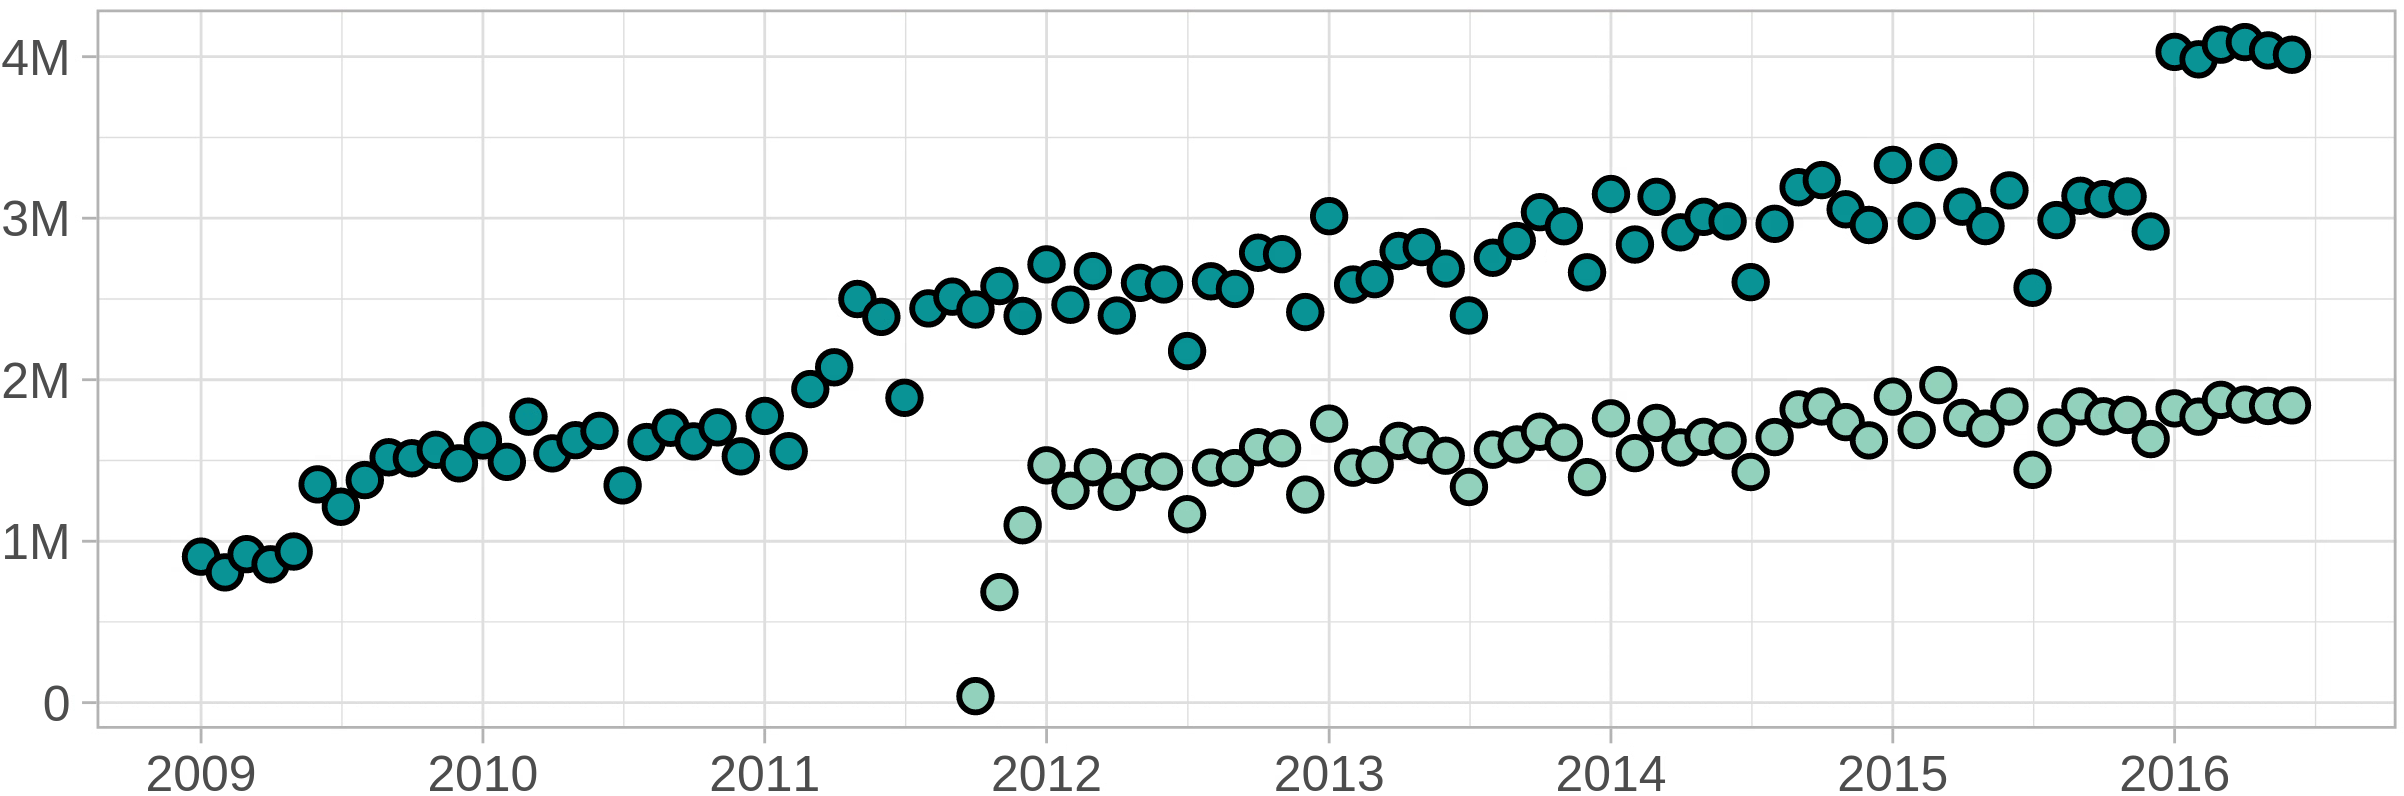
\includegraphics[width=\textwidth]{graphics/bth-biochem}
    \caption{%
        Monthly number of laboratory measurements in \acf*{BTH}
        originating from 
        (\,\cbox{color2}{\phantom{a}}\,) the \acs*{LABKA} and 
        (\,\cbox{color3}{\phantom{a}}\,) the \acs*{BCC} laboratory systems
        used in the Capital Region and Region Zealand respectively.
    }
    \label{fig:biochem-overview}
\end{figure}% ←

The laboratory tests results in the database is registered using
the \ac{NPU} system, which is an international terminology
curated and maintained by a commitee operating under 
\ac{IUPAC} and \ac{IFCC}.
~\autocite{arendtExisting2020}
The \ac{NPU} terminology is analagous to the 
\ac{LOINC} which have been widely adopted in several countries,
including the United States, Switzerland, Australia, and Germany.
~\autocite{mcdonaldLOINC2003}

\subsection{Patient Notes}

An important hallmark of the \ac{BTH} project
is its inclusion of an extensive corpus of unstructured clinical text.
This corpus comprises \num{74336119} unique entries,
spanning from 2006 to 2017, 
with notably lower number of entries from 2006 to 2009,
as illustrated in \cref{fig:notes-overview}.

% figure: bth notes stats→
\begin{figure}
    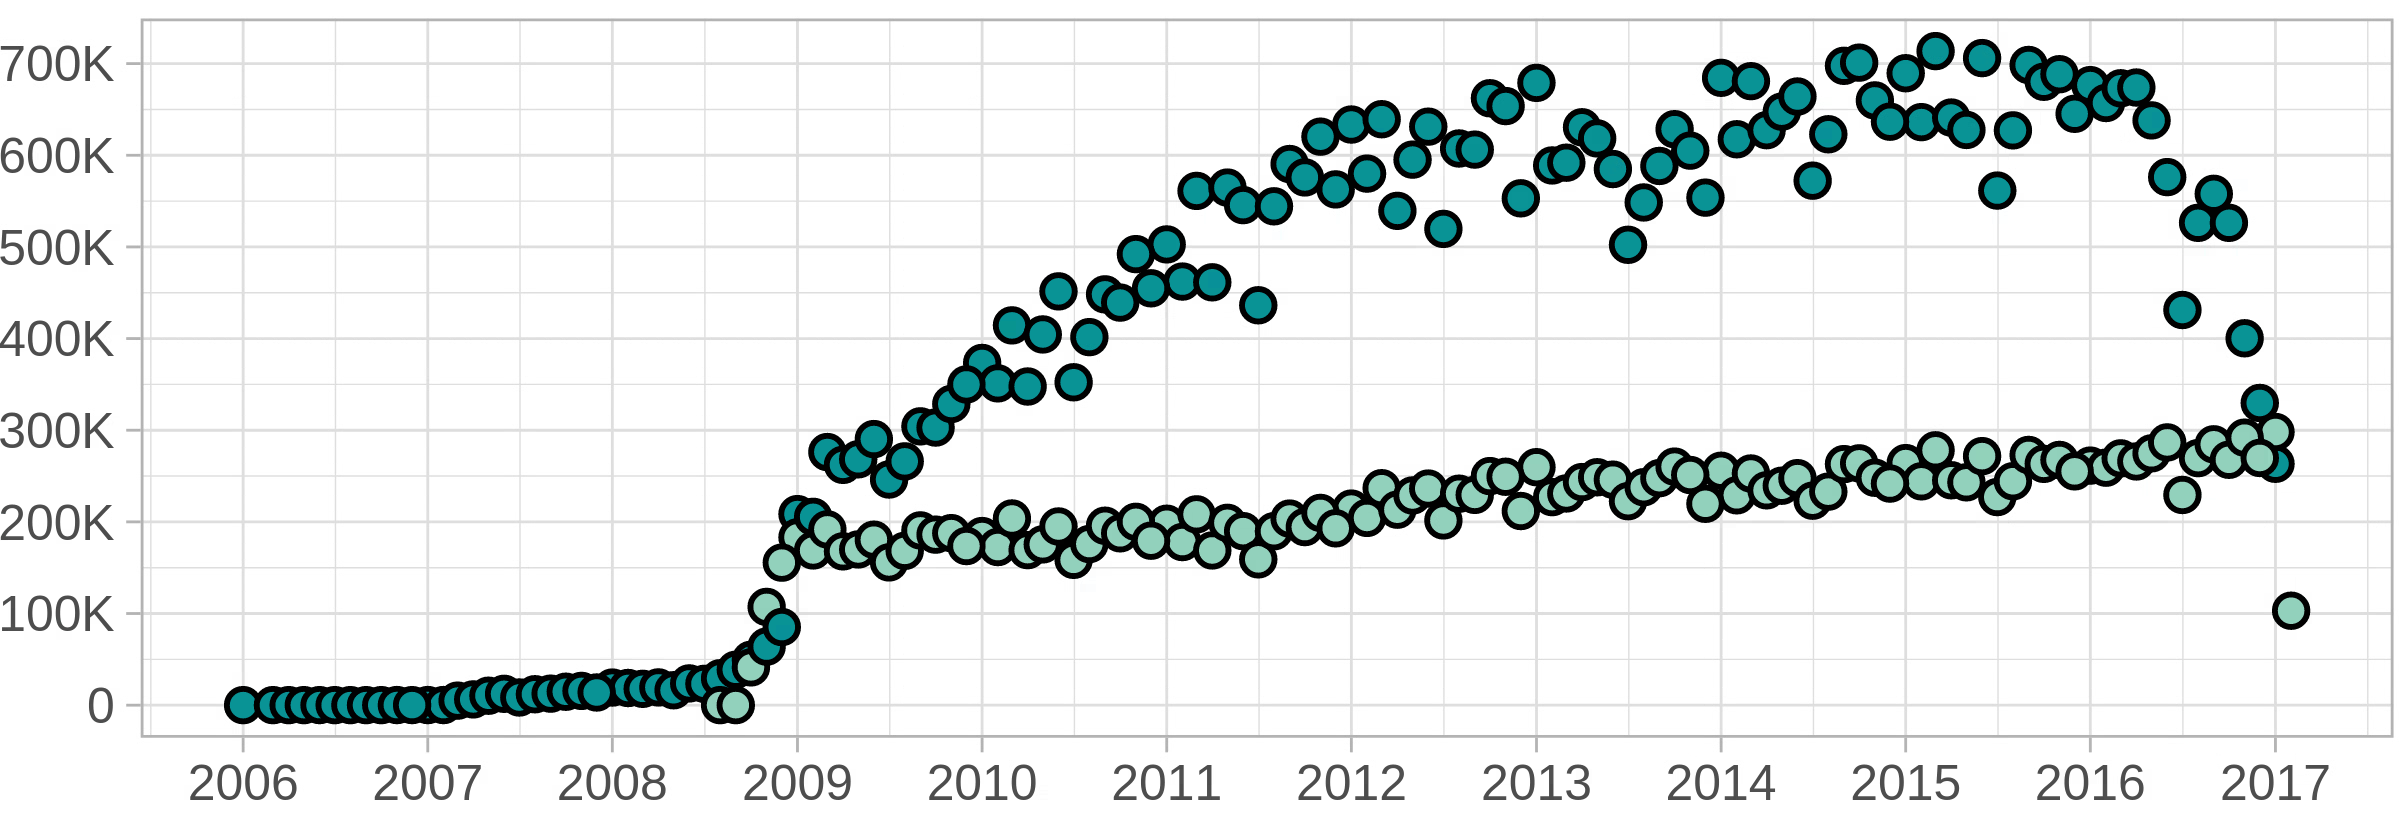
\includegraphics[width=\textwidth]{graphics/bth-notes}
    \caption{%
        Monthly number of clinical notes in \acf*{BTH}
        originating from 
        (\,\cbox{color2}{\phantom{a}}\,) the Capital Region hospitals and 
        (\,\cbox{color3}{\phantom{a}}\,) the Region Zealand hospitals.
    }
    \label{fig:notes-overview}
\end{figure}% ←

Originally, these clinical notes serve to meticulously record 
the individual patient's healthcare trajectory, detailing symptoms, 
observations by medical professionals, test results, 
and treatment responses.
While such data is not initially intended for research,
a main objective of the \ac{BTH} project was to harness
these notes as a rich source of phenotypic data,
crucial for the advancement of precision medicine.

As detailed in the review by \textcite{jensenMining2012}, 
clinical text represents the most challenging \ac{EHR} data modality for 
computational analysis, since it is inherently non-structured.
Deriving structured information from written text generally involves the
use of \ac{NLP} methods.
~\autocite{jensenMining2012}

One such method is \ac{NER}, a type of information extraction 
used in \ac{NLP} that involves identification and classification 
of predefined entities, typically recorded in large dictionaries
of known \enquote{concepts}.
In the context of clinical text,
entities could include diagnoses, symptoms, and medication
as illustrated in \cref{fig:notes-example}.
Current and prior members in the Brunak group 
have used \ac{NER} in many applications, 
for example,
\textcite{sorupSex2020},
\textcite{hjaltelinPancreatic2023},
and  
\textcite{kirkLinking2019}.

However, one important feature missing from these earlier applications 
is extraction of key--value pairs;
as also highlighted in \cref{fig:notes-example}, 
a typical clinical note can contain
semi-structured stretches of text,
with strings such as \enquote{blood pressure is 149/91}
or \enquote{bmi=25.2}.
To extract this clinically highly-relevant data,
I have as side-project developed an approach based 
on regular expressions for such key--value extraction.
Regular expressions, or regexes in short, 
is a type of concise metalanguage 
that specifies a search pattern for text.
~\autocite{Regular2023}

Using an iterative process, 
I constructed detailed regular expressions to 
extract blood pressure, height, weight, body-mass index, pack-years,
pulse, and temperature from the large \ac{BTH} corpus 
with high specificity.

We have not yet decided if this approach should be published,
and no manuscript detailing its development is therefore included here.
The underlying idea is neither novel,
see e.g. \textcite{turchinUsing2006} for a very similar example,
nor particularly interesting.
However, we found it to be surprisingly useful as a data-resource
for ongoing research projects.
As such, the clinical information extracted using this approach
have been utilized as prognostic factors in \studyii{} and \studyiii{}.

% figure: journal text→
\begin{figure}
{%
\newcommand{\diag}[1]{\cbox{color3!60!white}{#1}}
\newcommand{\symp}[1]{\cbox{color4!60!white}{#1}}
\newcommand{\drug}[1]{\cbox{color5!60!white}{#1}}
\newcommand{\quan}[1]{\cbox{color6!60!white}{#1}}
\newcommand{\kwpa}[1]{\cbox{color7!60!white}{#1}}

\begin{Verbatim}[commandchars=\\\{\}, fontsize=\scriptsize, 
    frame=single, framesep=1em, numbers=left, numbersep=3pt]
68-year-old woman, no earlier known cardiovascular disease, 
referred by gp for observation of \diag{angina pectoris}.

Risk factors:
\diag{Hypertension}: Yes, newly discovered, currently well-treated.
\diag{Hypercholesterolemia}: Yes. Under treatment.
Family: No family history of \diag{ischemic heart disease}.
Smoking: Quit 15 years ago, before that 20 pack-years.
Claudication: No.

Previously:
Known since 2001 with \diag{type II diabetes mellitus}, treated 
with \drug{Metformin}.  Followed up with regular checks. 
Complications with discrete neuropathy and beginning 
macular degeneration.

Currently:
For about 3 months, \symp{intermittent pressure in the left side}
\symp{of the chest}. No radiation, independent of physical 
activity. Daily attacks lasting a few seconds. During the 
same period, has been diagnosed with \diag{severely elevated blood}
\diag{pressure}. Recently started anti-hypertensive treatment with
good effect.

Medication:
- \drug{Metformin} \quan{1000 mg} x 2
- \drug{Simvastatin} \quan{20 mg} x 1
...

Objective:
Normal general condition.
Nutritional status above average.
\kwpa{Blood pressure 149/91}, \kwpa{pulse 76}, \kwpa{height 177 cm}, \kwpa{weight 96 kg}
\end{Verbatim}
\caption{Artificial example of unstructured text in an \ac{EHR}}
\label{fig:notes-example}
}
\end{figure}% ←
